yeoman: yo, bower, grunt

%Yeoman is an open source client-side development stack, consisting of tools and frameworks intended to help developers quickly build high quality web applications. Yeoman runs as a command-line interface written in Node.js which combines several functions into one place, such as generating a starter template, managing dependencies, running unit tests, providing a local development server, and optimizing production code for deployment.
%Yeoman was released at Google I/O 2012.

%Yeoman combines several popular open source tools in an attempt to streamline many aspects of the web development process.
%Using a "generator" concept inspired by Ruby on Rails,[2] Yeoman first creates a basic project structure with vendor libraries included. The most basic Yeoman generator supplies the HTML5 Boilerplate, Normalize.css, the jQuery JavaScript library, and Modernizr as a basic template for developers. Yeoman also runs interactively, asking the developer if they would like additional components such as Twitter Bootstrap or RequireJS (a library to support Asynchronous Module Definition) included. More sophisticated generators exist, such as ones which scaffold out a client-side MVC (Model-View-Controller) framework, such as the AngularJS or Backbone JavaScript libraries. Yeoman is meant to be modular such that anyone can design a generator to create a template for a particular type of project.[3]
%Beyond providing a template to quickly scaffold projects, Yeoman also helps with intermediary phases of web application development. Yeoman lints code for potential problems using JSHint, runs unit tests, and provides a development server for working on an application. Finally, Yeoman also offers a build automation process featuring optimizations such as minification and concatenation of script files. All of these features use pre-configured tasks for the Grunt JavaScript task runner.
%Yeoman is an open source project whose code is hosted on GitHub.[4] Several primary contributors are on the Google Chrome Developer Relations team, such as Addy Osmani, Paul Irish, and Eric Bidelman.[5] Contributors must sign a Contributor License Agreement before submitting code to the project to ensure that Google has the right to release their code under a BSD license.[6]


\begin{figure}[h]
\centering
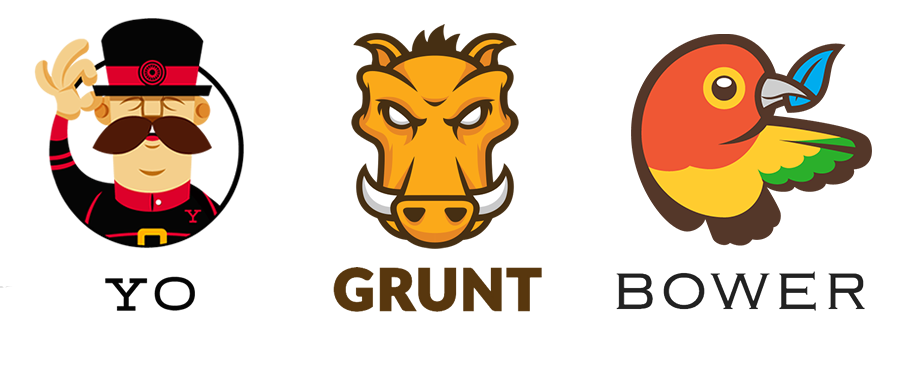
\includegraphics[width=0.7\linewidth]{./img/yo-grunt-bower.png}
\caption[I loghi di Yo, Grunt e Bower]{I loghi di Yo, Grunt e Bower}
\label{fig:yo-grunt-bower}
\end{figure}

\begin{figure}[h]
\centering
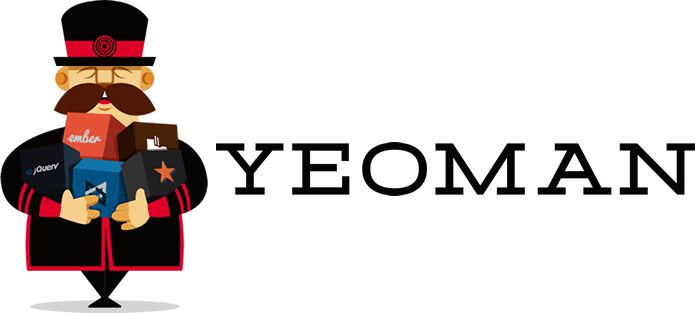
\includegraphics[width=0.7\linewidth]{./img/yeoman.png}
\caption[Il logo di Yeoman]{Il logo di Yeoman}
\label{fig:yeoman}
\end{figure}